\documentclass[12pt]{scrreprt}

\usepackage{fontspec}
\setmainfont{Times New Roman}

\usepackage{graphicx}
\usepackage{hyperref}
\usepackage{float}
\usepackage{geometry}
\geometry{a4paper, margin=1in}

\usepackage{titlesec} % Include titlesec package for custom section formatting
\titleformat{\section}[block]{\normalfont\Large\bfseries}{\thesection}{1em}{}
\titleformat{\subsection}[runin]{\normalfont\small\bfseries}{\thesubsection}{1em}{}

\title{Travel Agency Website Development}
\author{}
\date{}

\begin{document}

\maketitle

\section{Introduction}
User-Friendly Platform: Easy travel package selection and secure bookings.  
Seamless Booking: Customizable options for flights, hotels, and payments.  
Admin Management: Admins can manage packages and tour guide details.  
Market Demand: Driven by the growing need for modern online travel services.  
Comprehensive Solution: Covers user interface, payment gateway, and admin panel.

\section{Problem Statement}
Current Challenges: Travel agencies face inefficiencies, errors, and poor customer experience due to outdated booking methods.  
Lack of Integration: Existing systems lack seamless integration between package selection, customization, and payment processing.  
Admin Management Issues: Administrative tasks related to package and tour guide management are often cumbersome.  
Proposed Solution: A fully integrated Travel Agency website to streamline browsing, customization, and secure payment.  
Improved Efficiency: The project aims to enhance the booking experience for both customers and administrators.

\section{Objective}
\subsection{User-Friendly Interface}
\begin{itemize}
    \item Develop a responsive interface for browsing, selecting packages, and secure payments.
    \item Achieve 90\% user satisfaction, completing within 2 months.
\end{itemize}

\subsection{Secure Payment Gateway}
\begin{itemize}
    \item Integrate a reliable payment system like Stripe or PayPal.
    \item Ensure 95\% success in transactions, complete within 3 months.
\end{itemize}

\subsection{Admin Panel for Management}
\begin{itemize}
    \item Build an admin interface for managing packages and tour guide details.
    \item Support at least 50 packages, complete within 4 months.
\end{itemize}

\subsection{System Scalability \& Performance}
\begin{itemize}
    \item Optimize the backend to handle high traffic and data.
    \item Achieve load times under 2 seconds and handle 500 users, completing in the final month.
\end{itemize}

\subsection{User Testing \& Feedback}
\begin{itemize}
    \item User testing was conducted with 30 participants to gather feedback.
    \item Improve the system based on 80\% of user suggestions, completed in the last 2 weeks.
\end{itemize}

\section{Methodology}
\begin{itemize}
    \item Define Functional and Non-Functional Requirements: Clearly specify essential features like user registration, package selection, payment integration, and admin management, along with performance, security, and usability expectations.
    \item Conduct Feasibility Studies: Assess technical, operational, and economic feasibility to ensure the project’s resources, user acceptance, and cost-effectiveness.
    \item Analyze Existing Systems: Evaluate current travel agency systems to identify gaps, limitations, and areas for improvement.
    \item Implement Using Next.js and Laravel: Develop the website using Next.js for frontend and Laravel for backend, ensuring a robust and scalable solution.
    \item Design System Architecture: Develop a high-level architecture that defines core features, backend processes, and system flow, ensuring a scalable and efficient solution.
\end{itemize}

\vspace{1cm}

\section{Requirement Identification}
\begin{figure}[H]  % Use 'H' to fix the image position
    \centering
    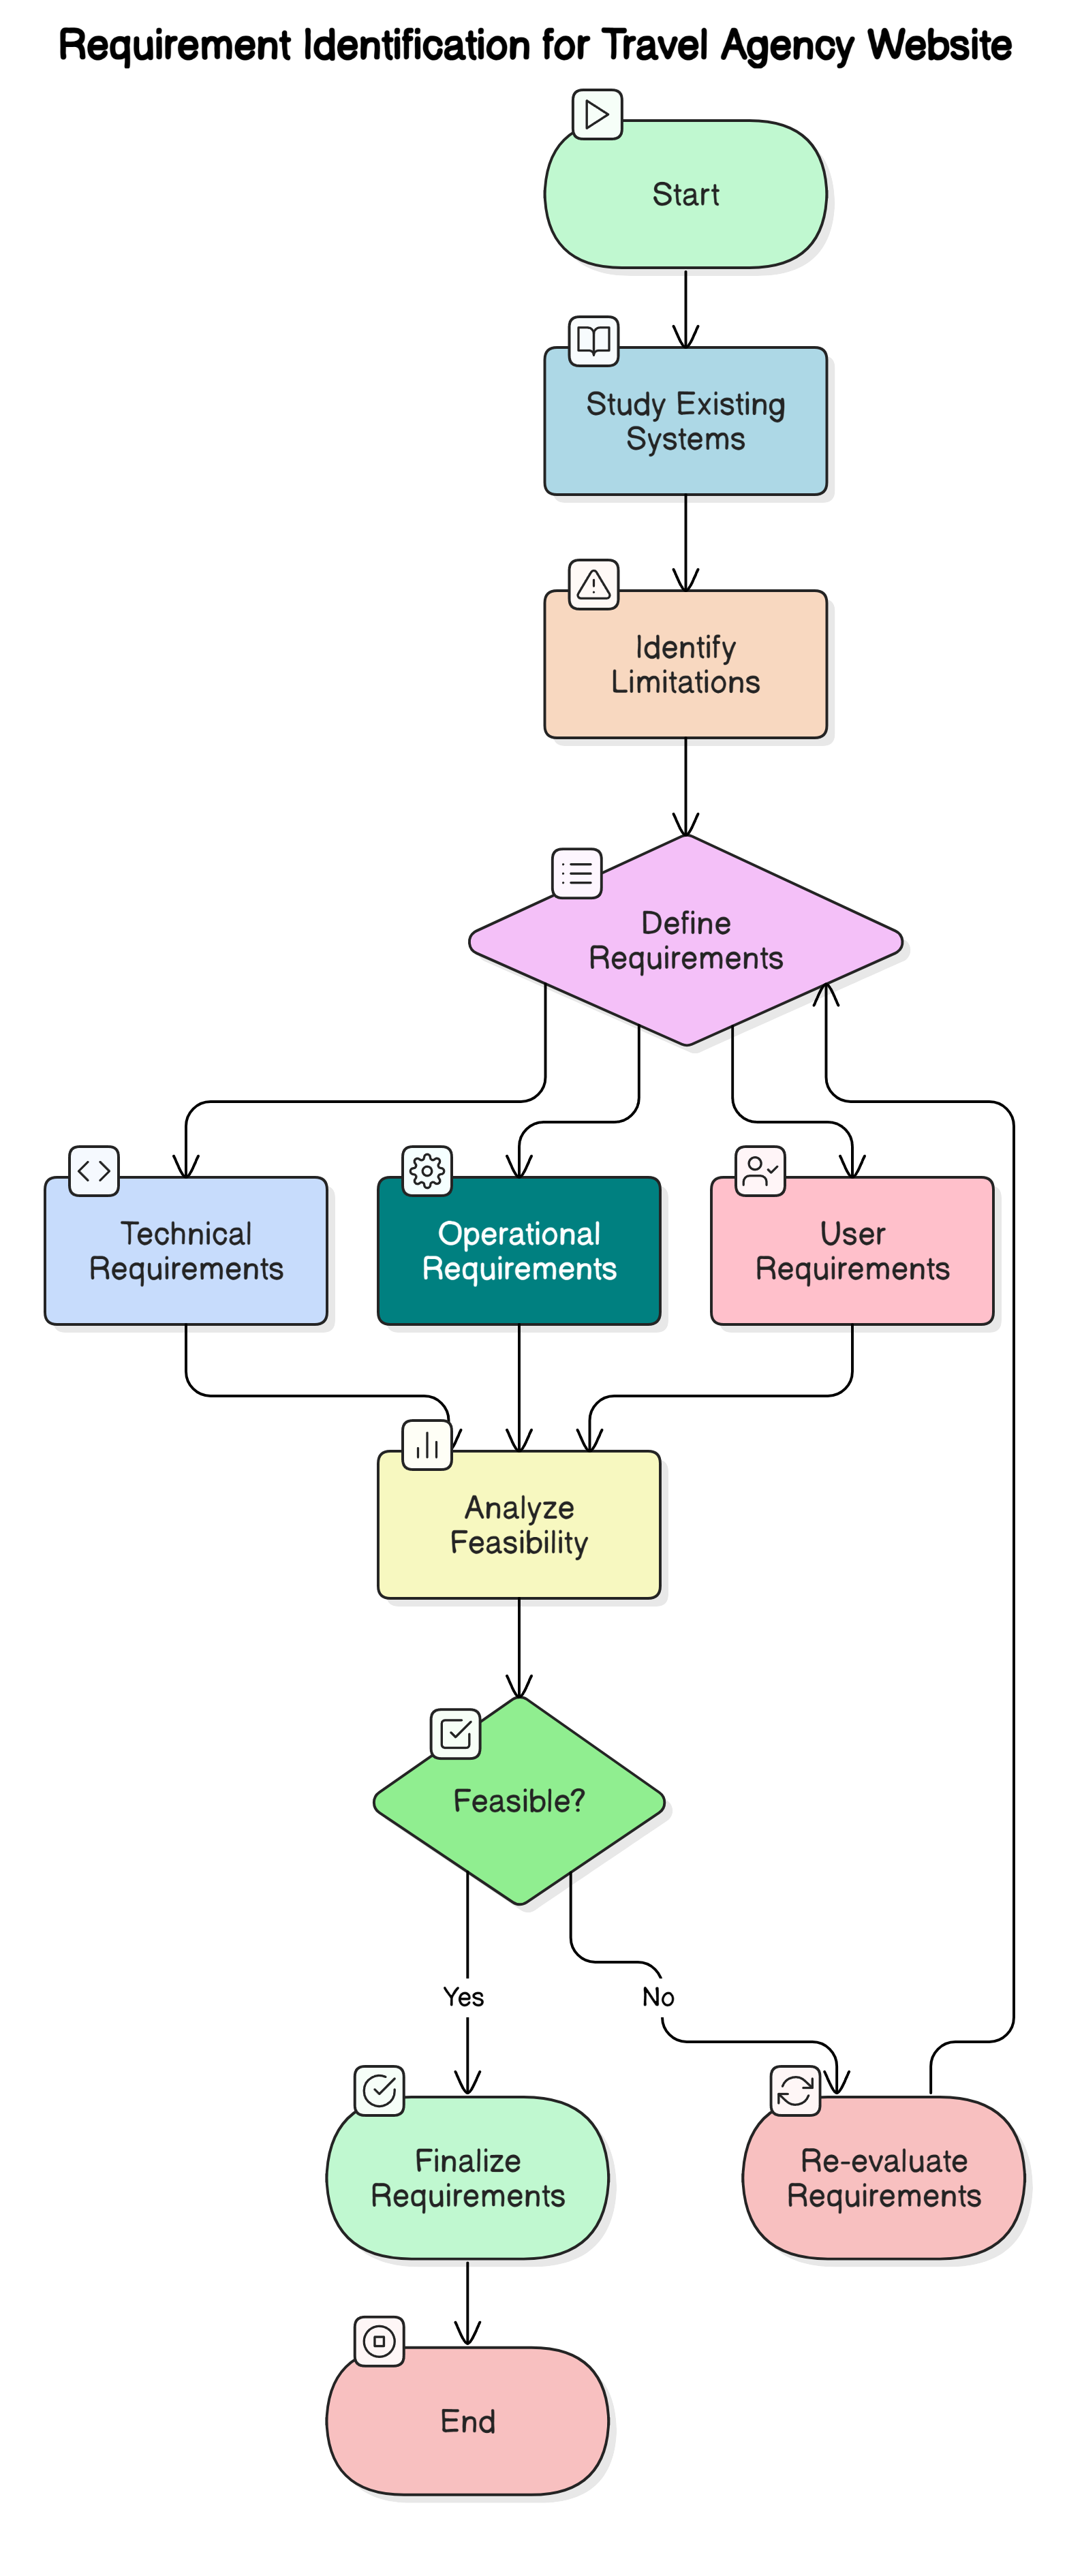
\includegraphics[width=0.5\linewidth]{flow.png}
    \caption{Requirement Identification Flowchart}
    \label{fig:Requirement Identification Flowchart}
\end{figure}

\section{Functional Requirements}
\subsection{User Features}
\begin{itemize}
    \item Browsing and Selecting Packages: Users can view and choose from a variety of travel packages.
    \item Customizing Travel Preferences: Users can select preferred flight and hotel types.
    \item Registration, Login, and Password Recovery: Secure user registration, login, and password recovery features.
    \item Responsive Design: Ensures seamless browsing on both desktop and mobile devices.
\end{itemize}

\subsection{System Features}
\begin{itemize}
    \item Secure Payment Processing: Integration of secure payment gateways for transaction handling.
    \item Monitor Bookings and User Data: Track user bookings and store relevant data for future interactions.
\end{itemize}

\subsection{Admin Features}
\begin{itemize}
    \item Manage Packages and Tour Guides: Admins can add, update, or delete travel packages and manage tour guide information.
    \item Package and Guide Information Management: Admins can efficiently manage and update the details of available packages and guides.
\end{itemize}

\section{Non-Functional Requirements}
\subsection{Performance}
\begin{itemize}
    \item Ensure the website loads in under 2 seconds and can handle over 500 concurrent users without performance degradation.
\end{itemize}

\subsection{Scalability}
\begin{itemize}
    \item Design the system to accommodate future growth in both users and data, ensuring it remains efficient as demand increases.
\end{itemize}

\subsection{Security}
\begin{itemize}
    \item Implement encryption and secure APIs to protect user transactions and sensitive data.
\end{itemize}

\subsection{Usability}
\begin{itemize}
    \item Provide an intuitive and user-friendly interface for both customers and administrators to ensure ease of use.
\end{itemize}

\subsection{Reliability}
\begin{itemize}
    \item Maintain an uptime of 99.9\%, with the ability to handle faults and errors gracefully to ensure consistent service.
\end{itemize}

\section{Algorithm}
Our system incorporates key algorithms to ensure a seamless booking experience. The Authentication Algorithm secures user access and manages sessions. The Package Selection Algorithm filters and optimizes package options based on user preferences. Lastly, the Payment Processing Algorithm handles secure transactions with third-party gateways. Together, these algorithms streamline the process, providing users with a smooth, efficient, and secure experience.

\section{Feasibility Analysis}
Our feasibility study shows that this project is both practical and achievable. Technically, we’ll use reliable tools like Next.js, Node.js, and MySQL, along with secure payment options like Stripe and PayPal. Operationally, the system will be easy to use, with a responsive design that works smoothly on both computers and mobile devices. Economically, it’s a smart investment, with costs of \$23,000 and benefits estimated at \$60,000, giving a net gain of \$37,000. The project will be completed in 10-12 weeks, following a clear plan with specific milestones. This study confirms the project’s potential to succeed.

\section{Conclusion}
To conclude, the proposed Travel Agency website will revolutionize the way users plan and book their trips. It offers a seamless, user-friendly platform that allows customers to browse, customize, and securely book their travel packages. On the administrative side, it automates key tasks, enabling efficient management of packages and tour guide details.  
By addressing traditional inefficiencies and enhancing accessibility, the system ensures a superior user experience while streamlining operations for the agency. This project not only demonstrates the potential of modern web technologies but also delivers a scalable solution that meets the needs of both users and administrators, paving the way for a more efficient and accessible travel booking experience.

\end{document}
